\documentclass{standalone}
\usepackage{tikz,ctex}
\usepackage{tikz-3dplot} % 2-1
\usepackage{unicode-math} % 2-5,4-1,4-2
\setmathfont{Fira Math Regular}
\setmainfont{Fira Sans}
\definecolor{background}{RGB}{239, 239, 239} % 4-5,6-2,6-5
\begin{document}
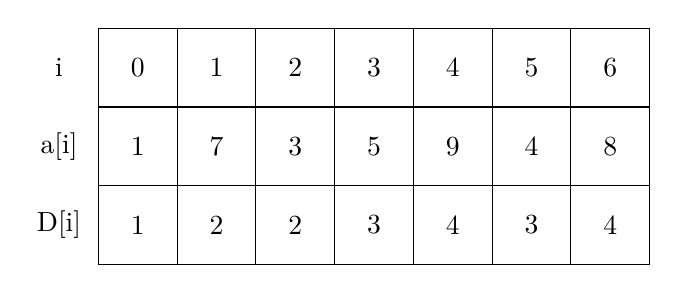
\begin{tikzpicture}
\foreach \x/\y/\num in {-1/0/D[i],-1/1/a[i],-1/2/i,0/0/1,1/0/2,2/0/2,3/0/3,4/0/4,5/0/3,6/0/4,0/1/1,1/1/7,2/1/3,3/1/5,4/1/9,5/1/4,6/1/8}{
    \node at (\x,\y) {\num};}
\foreach \x in {0,...,6}{
    \draw (\x,2) node{\x};}
\draw[xshift=-.5cm,yshift=-.5cm] (0,0) grid (7,3);
\end{tikzpicture}
\end{document}